\documentclass{article}
\usepackage[utf8]{inputenc}
\usepackage{amsthm}
\usepackage{hyperref}
\usepackage{pdfpages}
\begin{document}

\begin{titlepage}
    \begin{center}
        \vspace*{1cm}
            
        \Huge
        \textbf{Lab 9 Report}
            
        \vspace{0.5cm}
        \LARGE
        Analysis of the Chemical Composition of Various Cannabis Products
            
        \vspace{1.5cm}
            
        \textbf{Wenqi Guo*}, Austin and Mathew
        \begin{small}
            \url{https://scholar.google.com/citations?user=4YWcPZoAAAAJ}
        \end{small}

            
        \vfill
            
TA name:
Adebowale, Adeyemi

            
        \vspace{0.8cm}
            

            
        \Large
        Department of Chemistry\\
        University of British Columbia\\
        Dec 13, 2022
            
    \end{center}
\end{titlepage}
Code and raw \LaTeX \; of this lab report can be found on \url{https://github.com/weathon/Chem-Lab-9}
\section*{Abstract}
In this paper
\textbf{Keywords: } Cannabis, Statistcal Analysis, Dataset, Significance Analysis of Microarrays, Principal Component Analysis
\newpage
\section{Introduction}Materials and Methods
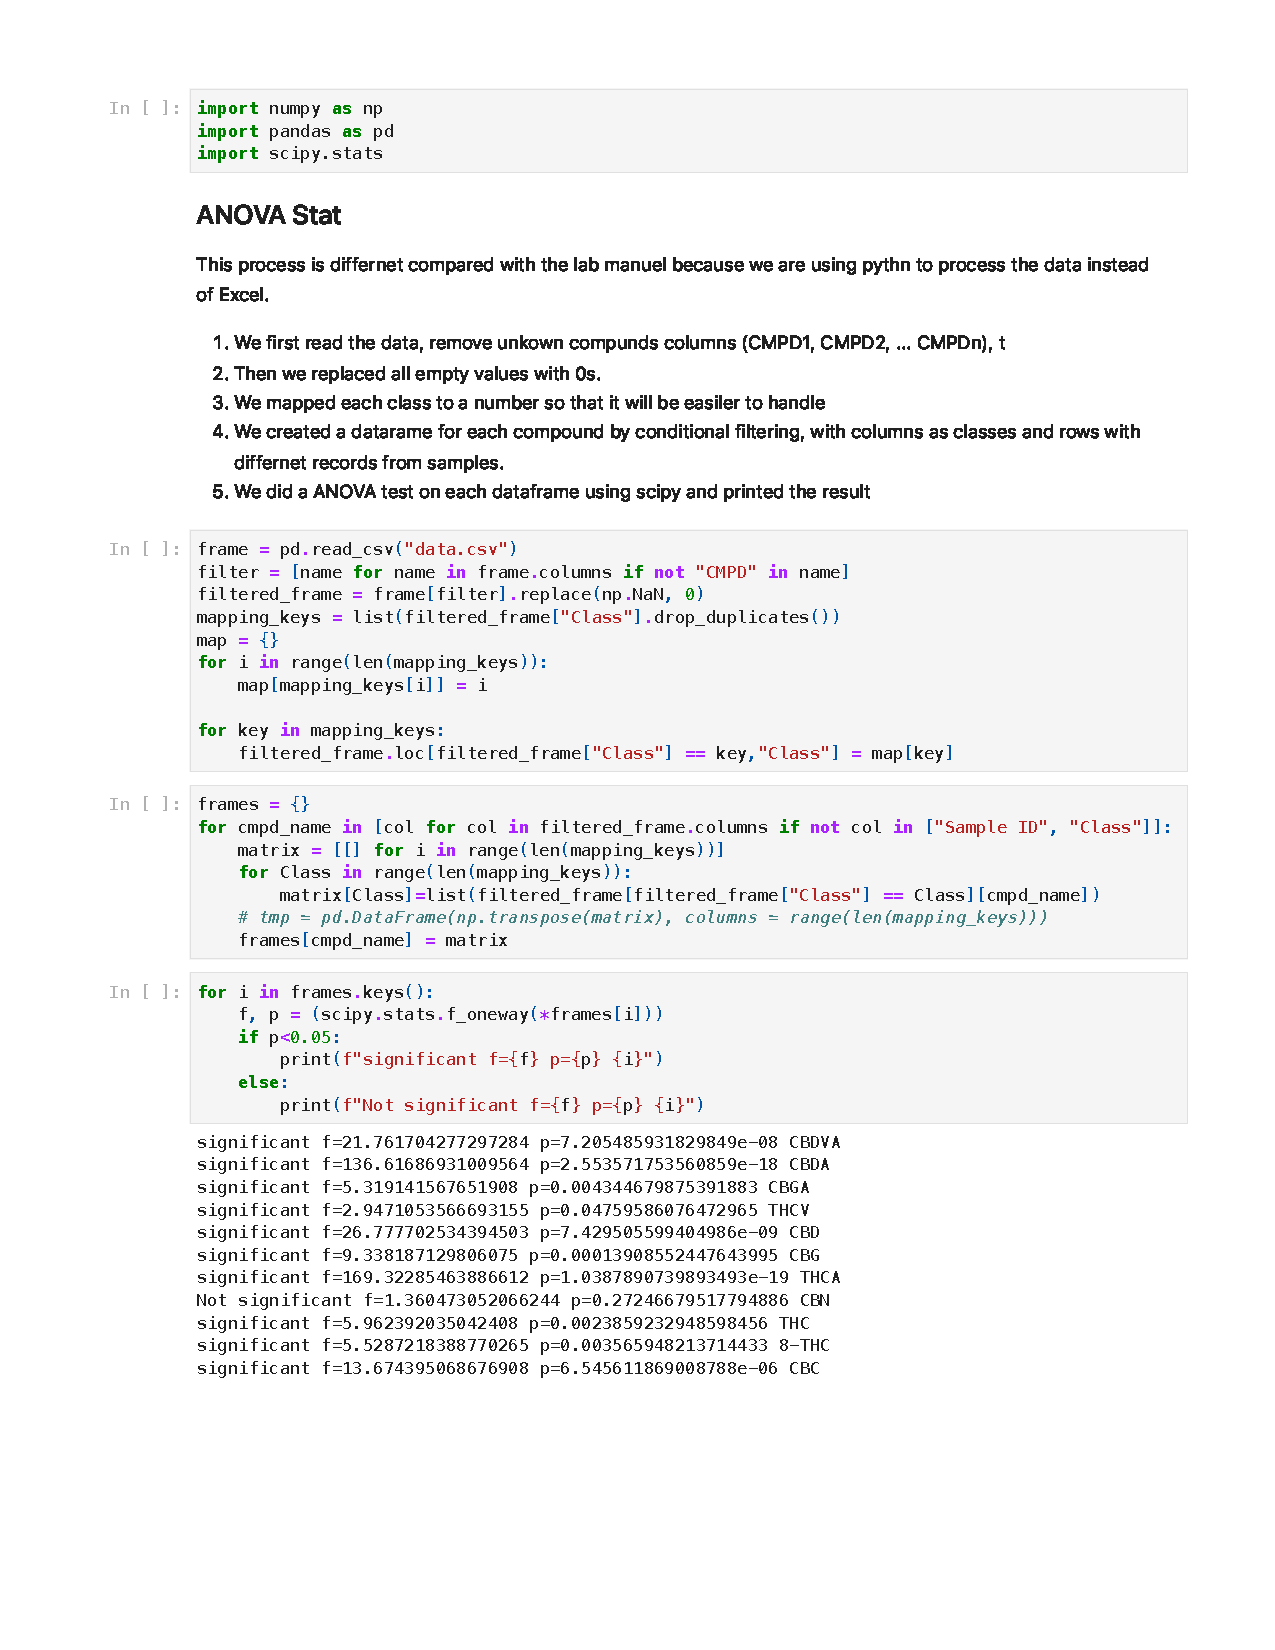
\includepdf[scale=0.8, offset=0 -1cm, pagecommand=\section{Materials and Methods}]{main.pdf}
\section{Result}
\section{Discussion}


\end{document}
